\chapter{Resultados}
\label{ch:resultados}
\section{Desempe\~no}
En esta secci\'on se describen los resultados obtenidos durante las experiencias de medici\'on de desempe\~no de la nueva versi\'on del programa en t\'erminos de tiempo y memoria principal usada. 
\bigskip

Las pruebas se realizaron usando el mismo conjunto de datos utilizado para medir el desempe\~no del programa original \ref{ch:prev_work}, adem\'as se emplearon como herramientas de medici\'on igualmente el perfilador de memoria \texttt{mem\_profiler} y la librer\'ia \textsc{Resource}\footnote{M\'etodo \texttt{get\_rusage}}.

\subsection{Filtros b\'asico y de m\'axima correntrop\'ia}

Los cuadros \ref{tab:t7} y \ref{tab:t9} muestran los resultados de tiempo medido en segundos de cada una de las partes del proceso de la rutina principal, para los tres datasets usando los filtros b\'asico y de m\'axima correntro\'ia, respectivamente. Posteriormente, los cuadros \ref{tab:t8} y \ref{tab:t10} resumen la totalidad de tiempo usado durante la ejecuci\'on (para ambos filtros). A todos estos resultados se les ha agregado la medici\'on de tiempo promedio utilizado por imagen (ya que las secuencias poseen largos diferentes). 

\begin{table}[h!]
\centering
\begin{tabular}{|l|l|l|l|l|}
\hline
\textbf{ID} & \textbf{C\'alc. Flujos [s]} & \textbf{Aplic. KF [s]} &  \textbf{Agrup. Pixeles [s]}  & \textbf{Obt. Candidatos [s]}\\ \hline \hline
SN14        & 285.81            & 22.45        &  65.18 & 0.00 \\ \hline
SN18            & 253.19             & 20.08         &  65.67  & 0.00\\ \hline
SN80            & 228.60             & 26.06         &   67.77 & 0.00 \\ \hline \hline
%Media & 303.08 &  26.23 & 37.83 & 0.01\\\hline 
$\bar{t}/Obs$ & 11.57 &  1.06 & 3.04 & 0.00\\\hline 
\end{tabular}
\caption{Tiempo de ejecuci\'on en segundos de cada proceso involucrado, usando el filtro de Kalman b\'asico refactorizado: c\'alculo de flujo estimaci\'on de filtros, agrupaci\'on de pixeles y obtenci\'on de candidatos (operaci\'on que involucra guardado de los mismos). La \'ultima fila describe el tiempo promedio que toma por observaci\'on (en segundos igualmente) para cada uno de los procesos. }
\label{tab:t7}
\end{table}


\begin{table}[h!]
\centering
\begin{tabular}{|l|l|}
\hline
\textbf{ID} & \textbf{Tiempo total} \\ \hline
\hline
SN14  & 373.44 \\\hline
SN18  & 338.94\\\hline
SN80  & 322.43 \\\hline\hline
%Media & 367.15 & 374.83 & 741.98  \\\hline
 $\bar{t}/Obs. $& 15.67 \\\hline 
\end{tabular}
\caption{Tiempo de ejecuci\'on de los procesos de b\'usqueda de supernova de HiTS, revisi\'on de los candidatos encontrados y tiempo total comprendido por ambos procesos usando filtro de Kalman B\'asico refactorizado. La \'ultima fila corresponde a tiempo total promedio por observaci\'on.}
\label{tab:t8}

\end{table}



\begin{figure}[h!]
\centering
\subfloat[Memoria ocupada en SN14]{\label{fig:new_kbf_14}{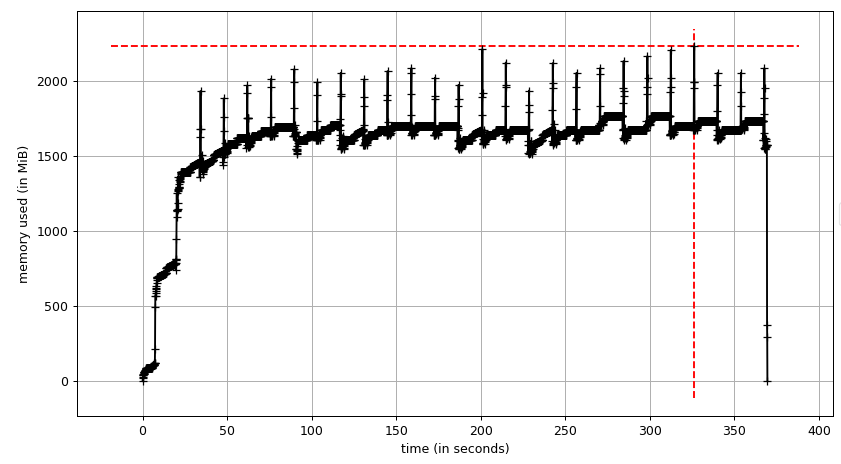
\includegraphics[width=0.5\textwidth]{images/results/sn14_new_bk}}}\hfill
\subfloat[Memoria ocupada en SN18]{\label{fig:new_kbf_18}{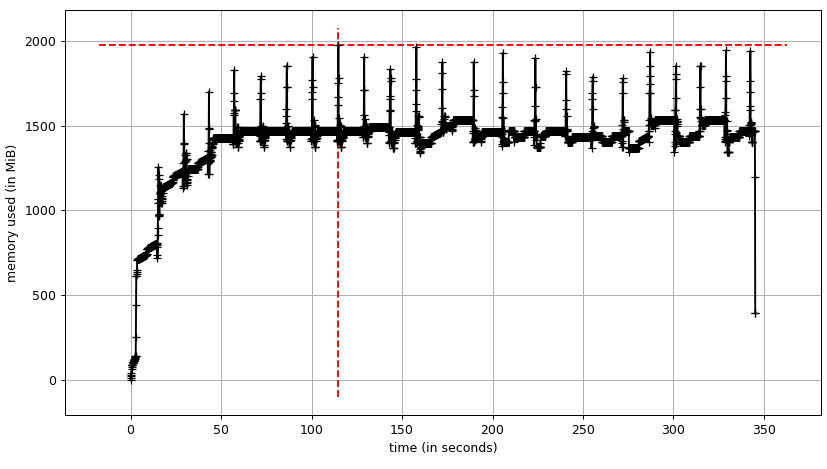
\includegraphics[width=0.5\textwidth]{images/results/sn18_new_bk}}}\vfill
\subfloat[Memoria ocupada en SN80]{\label{fig:new_kbf_80}{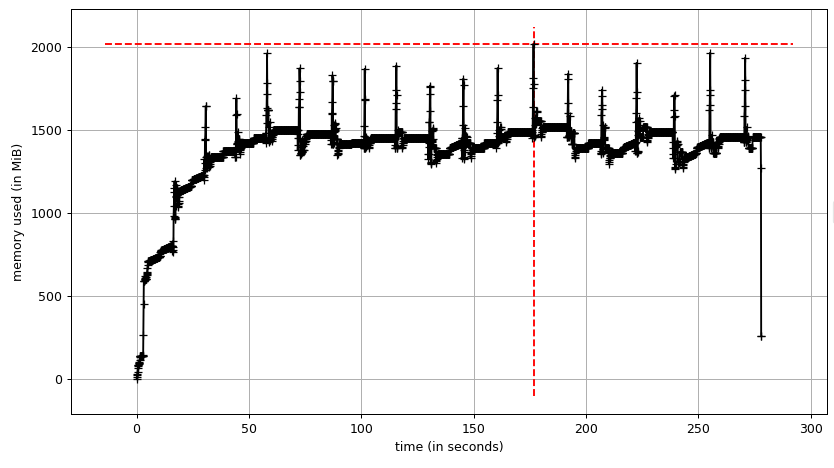
\includegraphics[width=0.5\textwidth]{images/results/sn80_new_bk}}}
\caption{Comportamiento de la memoria (en mebibytes) durante la ejecuci\'on para los tres conjuntos de datos. En los tres lanzamientos se us\'o el filtro de Kalman B\'asico.}
\label{fig:mem_new_kbf}
\end{figure}

\begin{table}[h!]
\centering
\begin{tabular}{|l|l|}
\hline
\textbf{ID} & Memoria [MB]\\\hline\hline
SN14 & 2098.00\\\hline
SN18 & 2066.72\\\hline
SN80 & 2119.24\\\hline
\end{tabular}
\caption{Memoria principal (en unidades de MB) usada durante la ejecuci\'on del programa refctorizado usando filtro de Kalman B\'asico.}
\label{tab:mem3}
\end{table}

\begin{table}[h!]
\centering
\begin{tabular}{|l|l|l|l|l|}
\hline
\textbf{ID} & \textbf{C\'alc. Flujos [s]} & \textbf{Aplic. KF [s]} &  \textbf{Agrup. Pixeles [s]}  & \textbf{Actual. Candidatos [s]}\\ \hline \hline
SN14        & 284.99            & 529.68        &  54.86 & 0.00 \\ \hline
SN18            & 256.58             & 507.46         &  66.73  & 0.00\\ \hline
SN80            & 209.02             & 411.94         &   45.94 & 0.00 \\ \hline \hline
%Media & 303.08 &  26.23 & 37.83 & 0.01\\\hline 
$\bar{t}/Obs$ & 11.00 &  0.97 & 2.24 & 0.00\\\hline 
\end{tabular}
\caption{Tiempo de ejecuci\'on en segundos de cada proceso involucrado, usando el filtro de Kalman de m\'axima correntrop\'ia refactorizado: c\'alculo de flujo estimaci\'on de filtros, agrupaci\'on de pixeles y obtenci\'on de candidatos (operaci\'on que involucra guardado de los mismos). La \'ultima fila describe el tiempo promedio que toma por observaci\'on (en segundos igualmente) para cada uno de los procesos. }
\label{tab:t9}
\end{table}

\begin{table}[h!]
\centering
\begin{tabular}{|l|l|}
\hline
\textbf{ID} & \textbf{Tiempo total} \\ \hline
\hline
SN14  & 869.53 \\\hline
SN18  & 830.77\\\hline
SN80  & 666.90 \\\hline\hline
%Media & 367.15 & 374.83 & 741.98  \\\hline
 $\bar{t}/Obs. $& 35.54 \\\hline 
\end{tabular}
\caption{Tiempo de ejecuci\'on de los procesos de b\'usqueda de supernova de HiTS, revisi\'on de los candidatos encontrados y tiempo total comprendido por ambos procesos usando filtro de Kalman de m\'axima correntrop\'ia refactorizado. La \'ultima fila corresponde a tiempo total promedio por observaci\'on.}
\label{tab:t10}
\end{table}

\begin{figure}[h!]
\centering
\subfloat[Memoria ocupada en SN14]{\label{fig:new_mcc_14}{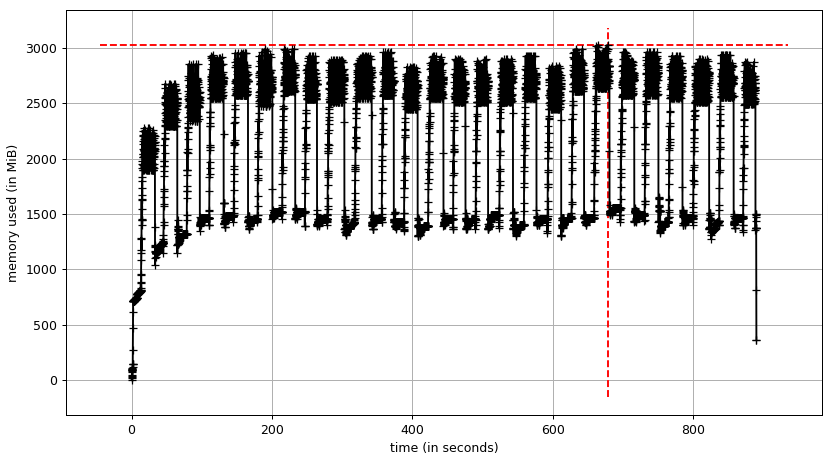
\includegraphics[width=0.5\textwidth]{images/results/sn14_new_mcc}}}\hfill
\subfloat[Memoria ocupada en SN18]{\label{fig:new_mcc_18}{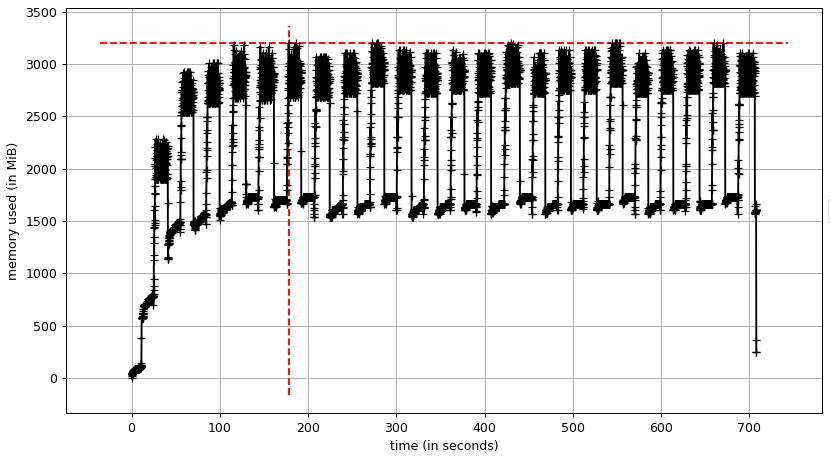
\includegraphics[width=0.5\textwidth]{images/results/sn18_new_mcc}}}\vfill
\subfloat[Memoria ocupada en SN80]{\label{fig:new_mcc_80}{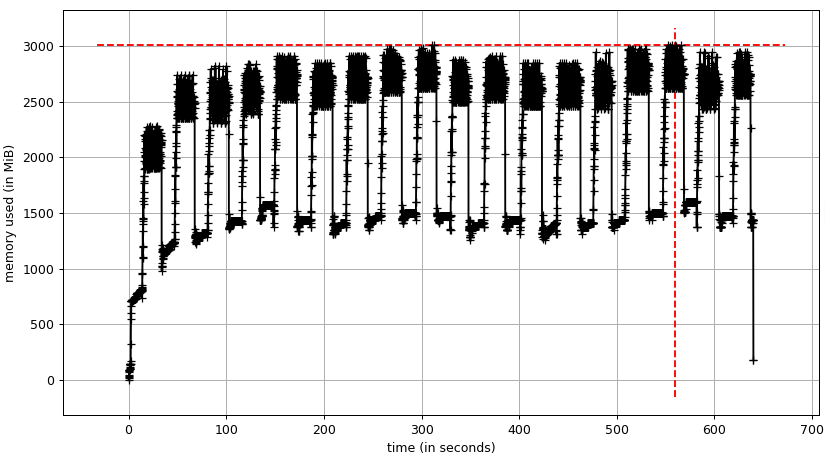
\includegraphics[width=0.5\textwidth]{images/results/sn80_new_mcc}}}
\caption{Comportamiento de la memoria (en mebibytes) durante la ejecuci\'on para los tres conjuntos de datos. En los tres lanzamientos se us\'o el filtro de Kalman de m\'axima correntrop\'ia.}
\label{fig:mem_new_kbf}
\end{figure}

\begin{table}[h!]
\centering
\begin{tabular}{|l|l|}
\hline
\textbf{ID} & Memoria [MB]\\\hline\hline
SN14 & 3164.83\\\hline
SN18 & 3186.06\\\hline
SN80 & 3154.98\\\hline
\end{tabular}
\caption{Memoria principal (en unidades de MB) usada durante la ejecuci\'on del programa refactorizado usando filtro de Kalman de m\'axima correntrop\'ia.}
\label{tab:mem4}
\end{table}

\subsection{Filtro unscented}
\section{Pruebas en Leftraru}
\subsection{Filtro b\'asico}
\subsection{Filtro de m\'axima correntrop\'ia}
\subsection{Filtro unscented}
